\documentclass[margin=5mm]{standalone}
\usepackage[dvipsnames]{xcolor}
\usepackage{pgfplots}
\usepackage{tikz}
\usepackage[tikz]{ocgx2}

\pgfplotsset{compat=1.18}
\begin{document}

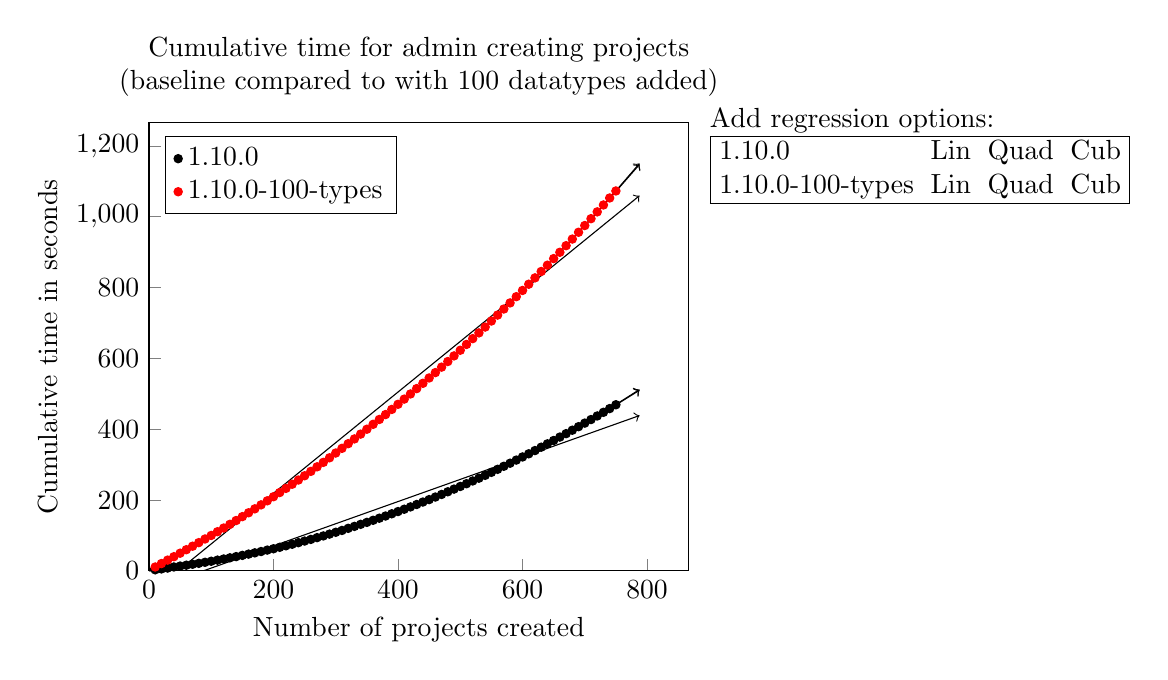
\begin{tikzpicture}
    \begin{axis}[
        align = center,
        legend pos = north west,
        legend cell align = left,
        xlabel = Number of projects created,
        ylabel = Cumulative time in seconds,
        xtick pos = left,
        ytick pos = left,
        scaled ticks = false,
        xmin = 0,
        ymin = 0,
        title = {Cumulative time for admin creating projects (baseline compared to with 100 datatypes added)},
        title style = {text width = 0.8\textwidth},
        legend entries={\switchocg{1.10.0}{1.10.0},\switchocg{1.10.0-100-types}{1.10.0-100-types}}]
        \begin{scope}[ocg = {ref = 1.10.0-Lin, status = invisible}]
            \plot[domain=0:788,->,forget plot] (\x,{-54.46349405405413079961363109759986400604248046875 + 0.625762668563300206159283334272913634777069091796875*(\x)^1});
        \end{scope}
        \begin{scope}[ocg = {ref = 1.10.0-Quad, status = invisible}]
            \plot[domain=0:788,->,forget plot] (\x,{3.87097021843742883362438078620471060276031494140625 + 0.17120840150492411257943103919387795031070709228515625*(\x)^1 + 0.000598097719813652927041414120168383306008763611316680908203125*(\x)^2});
        \end{scope}
        \begin{scope}[ocg = {ref = 1.10.0-Cub, status = invisible}]
            \plot[domain=0:788,->,forget plot] (\x,{2.50907278291968527383914988604374229907989501953125 + 0.192025809507216649318905865584383718669414520263671875*(\x)^1 + 0.000530070874882696452430608236028319879551418125629425048828125*(\x)^2 + 0.000000059672670992067038875635649926298942347102638450451195240020751953125*(\x)^3});
        \end{scope}
        \begin{scope}[ocg = {ref = 1.10.0, status = visible}]
            \addplot[
                only marks,
                color = black,
                mark = *,
                mark size = 1.5 pt
            ]coordinates {(10,3.229)(20,5.713)(30,8.155)(40,11.25)(50,13.765)(60,16.185)(70,18.851)(80,21.511)(90,24.409)(100,27.356)(110,30.522)(120,33.74)(130,37.053)(140,40.447)(150,43.945)(160,47.528)(170,51.066)(180,54.826)(190,58.848)(200,62.633)(210,66.784)(220,71.006)(230,75.329)(240,79.781)(250,84.395)(260,89.017)(270,94.024)(280,98.822)(290,104.006)(300,109.166)(310,114.299)(320,120.271)(330,125.771)(340,131.575)(350,137.076)(360,142.939)(370,148.839)(380,155.059)(390,161.352)(400,167.67)(410,174.172)(420,180.767)(430,187.56)(440,194.529)(450,201.425)(460,208.624)(470,215.913)(480,223.473)(490,231.031)(500,238.427)(510,246.208)(520,254.007)(530,261.821)(540,269.858)(550,278.346)(560,286.864)(570,295.467)(580,304.108)(590,312.919)(600,321.764)(610,330.663)(620,339.818)(630,349.374)(640,358.779)(650,368.187)(660,377.883)(670,387.56)(680,397.255)(690,407.23)(700,417.284)(710,427.347)(720,437.454)(730,447.772)(740,458.269)(750,469.103)};
        \end{scope}
        \begin{scope}[ocg = {ref = 1.10.0-100-types-Lin, status = invisible}]
            \plot[domain=0:788,->,forget plot] (\x,{-66.5159279279281321350936195813119411468505859375 + 1.42873303840682819298990580136887729167938232421875*(\x)^1});
        \end{scope}
        \begin{scope}[ocg = {ref = 1.10.0-100-types-Quad, status = invisible}]
            \plot[domain=0:788,->,forget plot] (\x,{5.4145132173265135833162275957874953746795654296875 + 0.86823609441783078377596893915324471890926361083984375*(\x)^1 + 0.00073749597893289146714745907473798069986514747142791748046875*(\x)^2});
        \end{scope}
        \begin{scope}[ocg = {ref = 1.10.0-100-types-Cub, status = invisible}]
            \plot[domain=0:788,->,forget plot] (\x,{3.435120553703845391879667658940888941287994384765625 + 0.89849228229273625512263379278010688722133636474609375*(\x)^1 + 0.000638625216514178417614999716533930040895938873291015625*(\x)^2 + 0.0000000867287389637834269361256998853715316499801701866090297698974609375*(\x)^3});
        \end{scope}
        \begin{scope}[ocg = {ref = 1.10.0-100-types, status = visible}]
            \addplot[
                only marks,
                color = red,
                mark = *,
                mark size = 1.5 pt
            ]coordinates {(10,11.141)(20,20.858)(30,30.568)(40,40.224)(50,50.109)(60,59.945)(70,69.776)(80,79.935)(90,90.201)(100,100.246)(110,110.72)(120,121.096)(130,131.586)(140,142.305)(150,153.318)(160,164.216)(170,175.292)(180,186.517)(190,197.942)(200,209.535)(210,221.293)(220,233.022)(230,244.787)(240,256.668)(250,268.683)(260,281.1)(270,293.898)(280,306.424)(290,319.394)(300,332.893)(310,346.062)(320,359.263)(330,372.644)(340,386.242)(350,399.992)(360,413.847)(370,427.583)(380,441.433)(390,455.894)(400,470.374)(410,485.051)(420,499.552)(430,514.66)(440,529.629)(450,544.722)(460,559.874)(470,575.289)(480,591.097)(490,607.036)(500,622.927)(510,639.391)(520,655.749)(530,671.966)(540,688.463)(550,705.472)(560,722.281)(570,739.34)(580,756.545)(590,774.182)(600,791.746)(610,809.361)(620,827.227)(630,845.262)(640,862.992)(650,881.657)(660,899.538)(670,918.133)(680,936.813)(690,955.996)(700,974.985)(710,994.333)(720,1013.574)(730,1033.024)(740,1052.763)(750,1072.541)};
        \end{scope}
    \end{axis}
    \begin{scope}
        \addtolength{\tabcolsep}{-0.3em}
        \node [below right, shape=rectangle, align=left](regressiontable) at (7,6) {
            Add regression options: \\
            \begin{tabular}{|llll|}
                \hline
                1.10.0 & \switchocg{1.10.0-Lin}{Lin} & \switchocg{1.10.0-Quad}{Quad} & \switchocg{1.10.0-Cub}{Cub} \\
                1.10.0-100-types & \switchocg{1.10.0-100-types-Lin}{Lin} & \switchocg{1.10.0-100-types-Quad}{Quad} & \switchocg{1.10.0-100-types-Cub}{Cub} \\
                \hline
            \end{tabular}
        };
    \end{scope}
\end{tikzpicture}

\end{document}